\section{Konfiguration der ET 200SP} \label{sec:Konfiguration_der_ET_200_SP}

\subsection{ET 200SP hinzufügen}
Über die \textbf{Netzsicht} im Katalog nach der Bezeichnung des \textbf{IM 155-Interfacemoduls} suchen (hier: IM 155-6PN HF (6ES7155-6AU00-0CN0)) und hinzufügen.\\
Pfad: Katalog > Dezentrale Peripherie > ET 200SP > Interfacemodule > PROFINET > IM 155-6 PN HF

\begin{figure}[H]
    \centering
   \begin{minipage}[b]{.4\linewidth}
        \centering
        \fbox{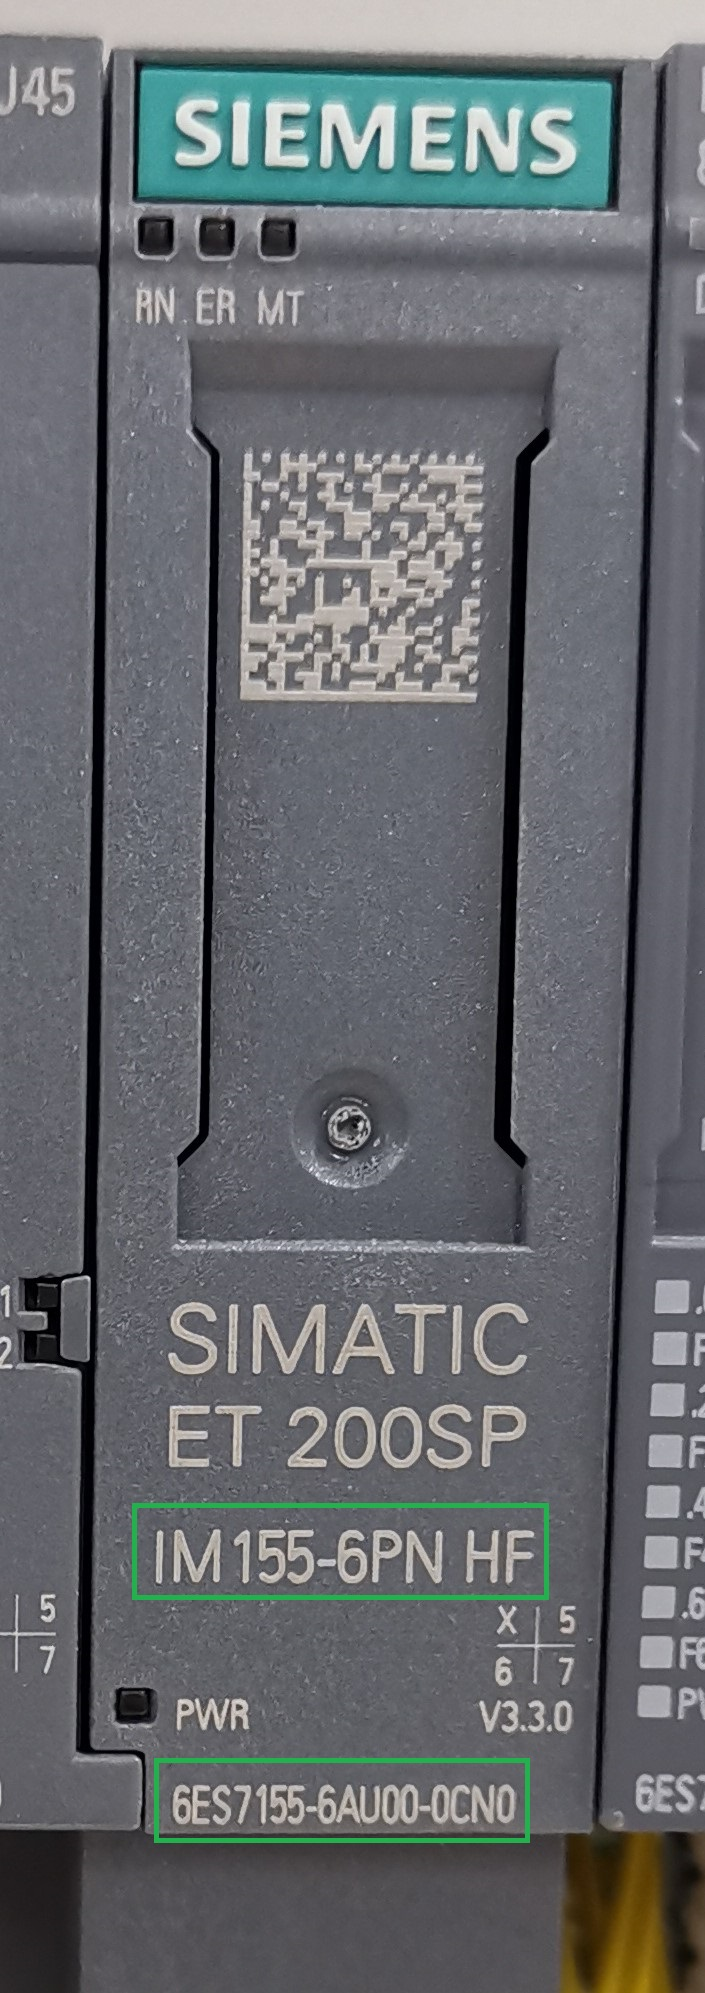
\includegraphics[width=0.4\linewidth]{Bilder/4. Konfiguration der ET 200 SP/4.1 ET 200 SP hinzufügen/(4.1.1) Modulbezeichnung am Beispiel des IM 155-Moduls.jpg}}
        \caption[Modulbezeichnung am Beispiel des IM 155-Interfacemoduls]{Modulbezeichnung am Beispiel des IM 155-Interfacemoduls}
        \label{fig:Bild4.1}
   \end{minipage}
   \hspace{.1\linewidth}% Abstand zwischen Bilder
   \begin{minipage}[b]{.4\linewidth}
        \centering
        \fbox{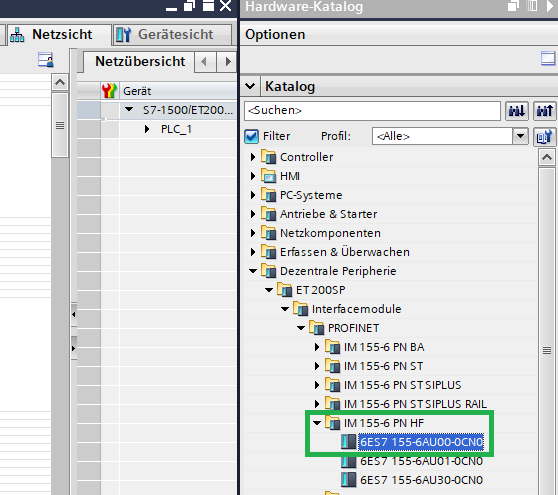
\includegraphics[width=1.1\linewidth]{Bilder/4. Konfiguration der ET 200 SP/4.1 ET 200 SP hinzufügen/(4.1.2) Dezentrale Peripherie hinzufuegen.png}}
        \caption[Dezentrale Peripherie hinzufügen]{Dezentrale Peripherie hinzufügen\\}
        \label{fig:Bild4.2}
   \end{minipage}
\end{figure}

\clearpage

\subsection{Module hinzufügen}
In der \textbf{Gerätesicht} der ET 200SP über den Katalog die weiteren Module hinzufügen.\\
\textbf{ACHTUNG:} Die Bezeichnungen auf den realen Modulen weichen teils von denen im TIA-Portal ab.

\begin{figure}[H]
   \centering
   \fbox{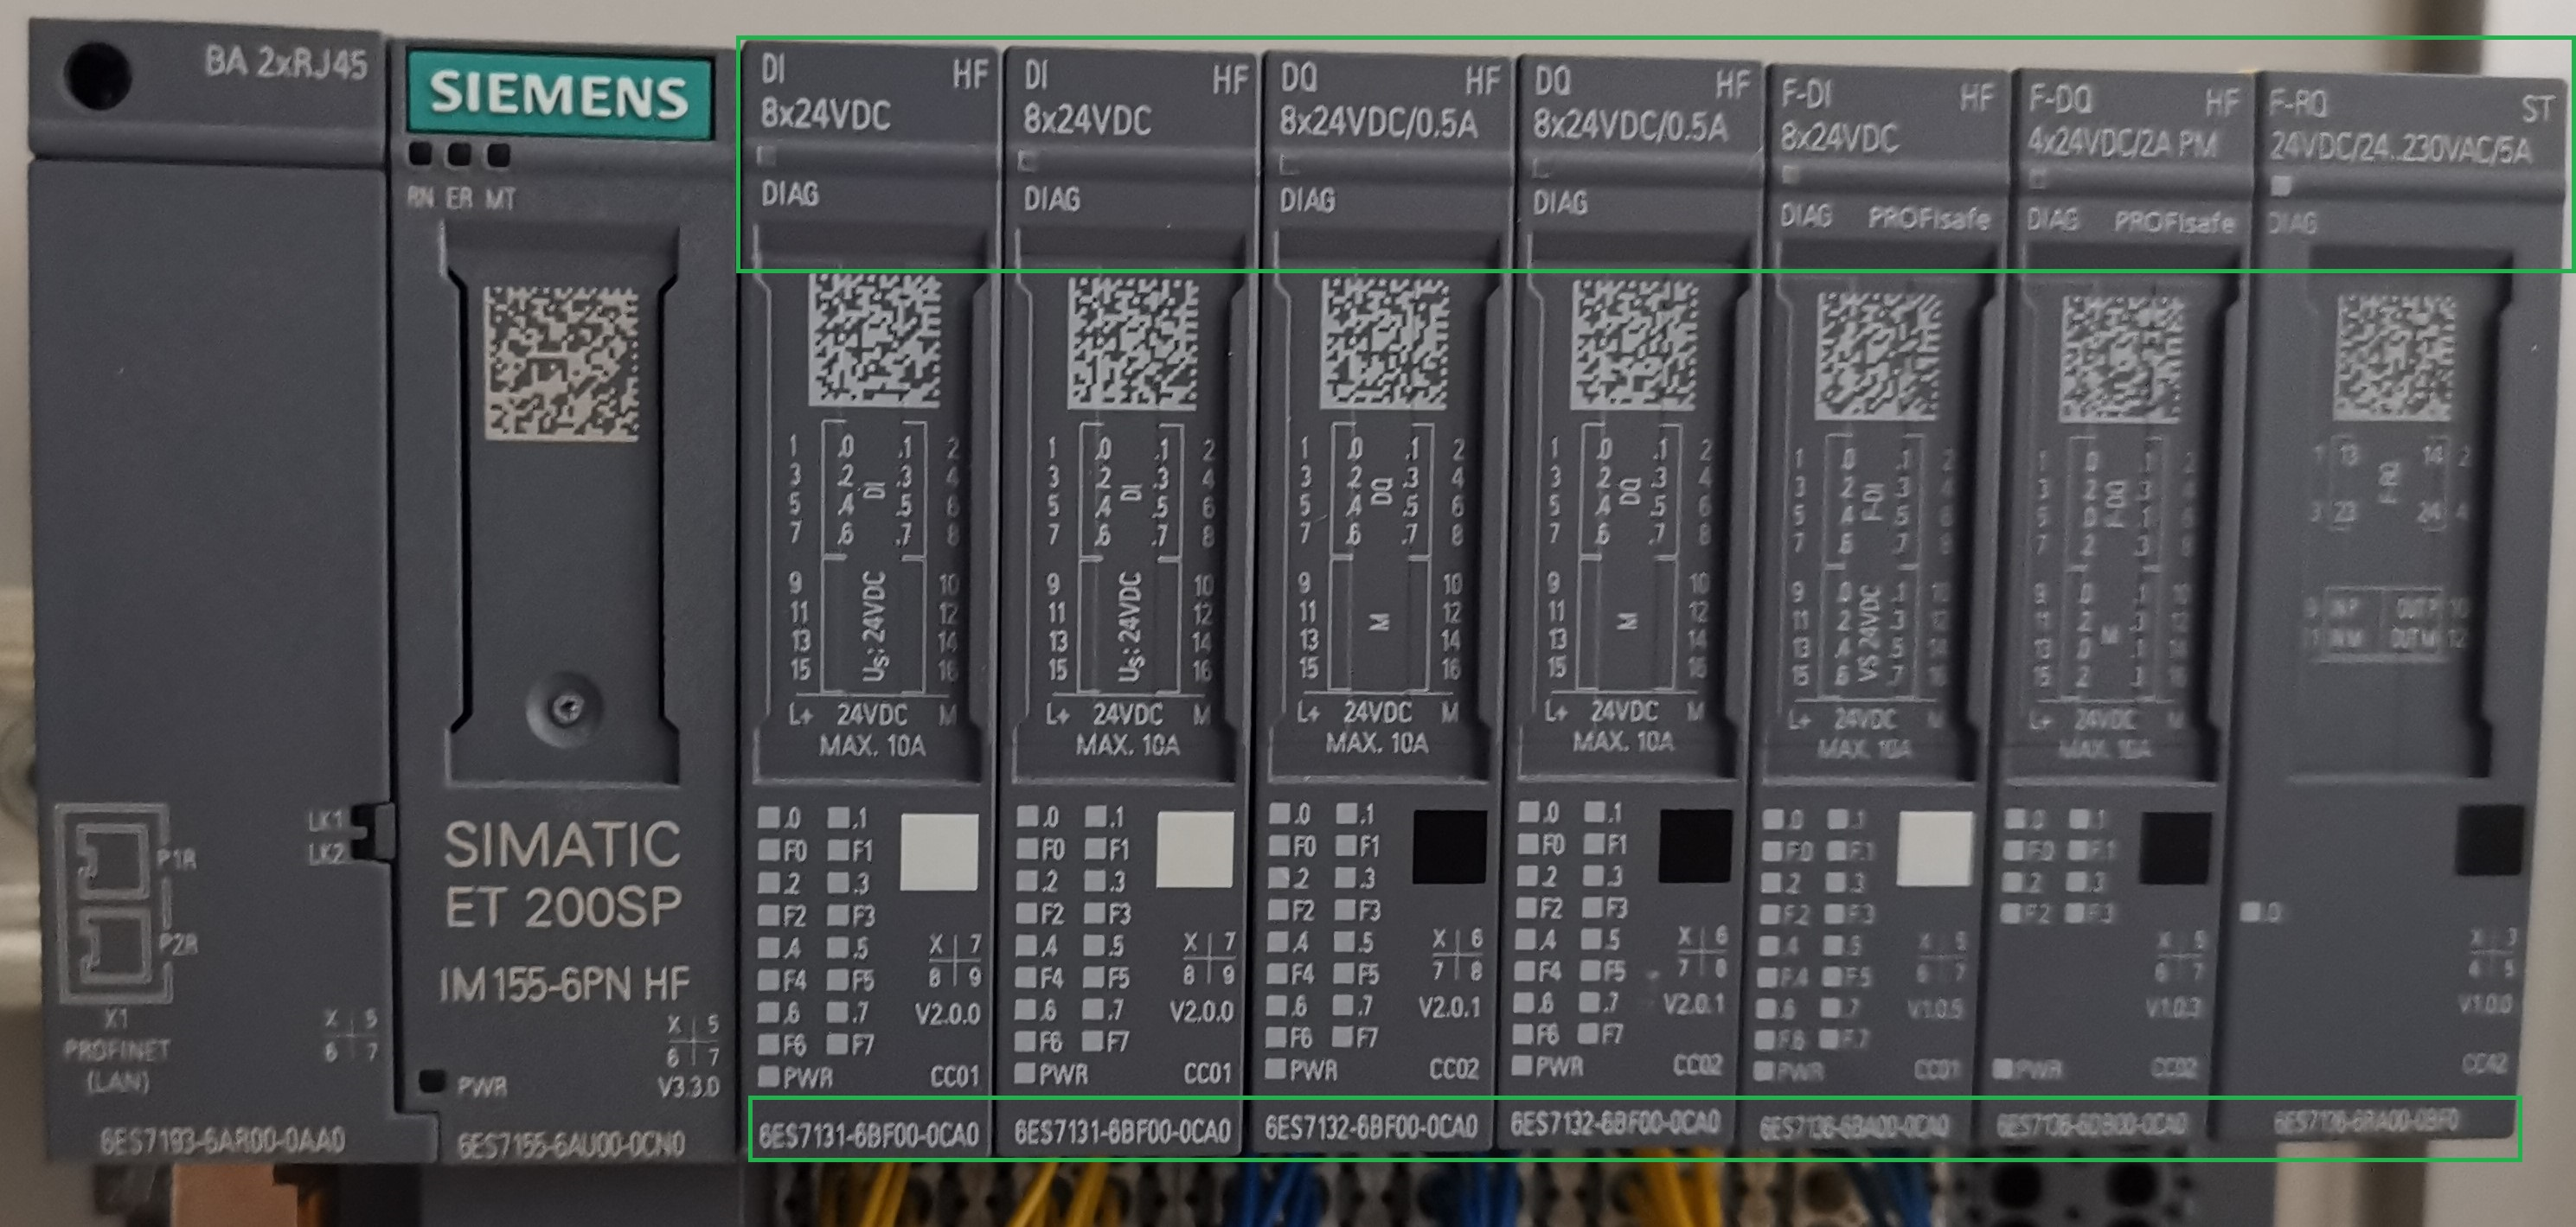
\includegraphics[width=0.9\textwidth]{Bilder/4. Konfiguration der ET 200 SP/4.2 Module hinzufügen/(4.2.1) Übersicht aller Module der dezentralen Peripherie.jpg}}
   \caption[Übersicht der Module der dezentralen Peripherie]{Übersicht der Module der dezentralen Peripherie}
   \label{fig:Bild4.3}
\end{figure}

\begin{table}[H]
    \centering
    \begin{tabular}{|c|c|c|}
        \hline
         \textbf{Modulbezeichnung} & \textbf{Modulnummer} & \textbf{Version} \\
         \hline
         DI 8x24VDC HF	& 6ES7131-6BF00-0CA0	& 2.0.0 \\
         \hline
         DI 8x24VDC HF	& 6ES7131-6BF00-0CA0	& 2.0.0 \\
         \hline
         DQ 8x24VDC/0.5A HF &	6ES7132-6BF00-0CA0	& 2.0.1 \\
         \hline
         DQ 8x24VDC/0.5A HF &	6ES7132-6BF00-0CA0	& 2.0.1 \\
         \hline
         F-DI 8x24VDC HF & 	6ES7136-6BA00-0CA0	& 1.0.5 \\
         \hline
         F-DQ 4x24VDC/2A PM HF & 	6ES7136-6DB00-0CA0	& 1.0.3 \\
         \hline
         F-RQ 24VDC/24…230VAC/5A ST & 	6ES7136-6RA00-09F0	& 1.0.0 \\
         \hline
    \end{tabular}
    \caption{Modulbezeichnungen, -nummern und -versionen}
    \label{tab:Tab4.1}
\end{table}

\begin{figure}[H]
   \centering
   \fbox{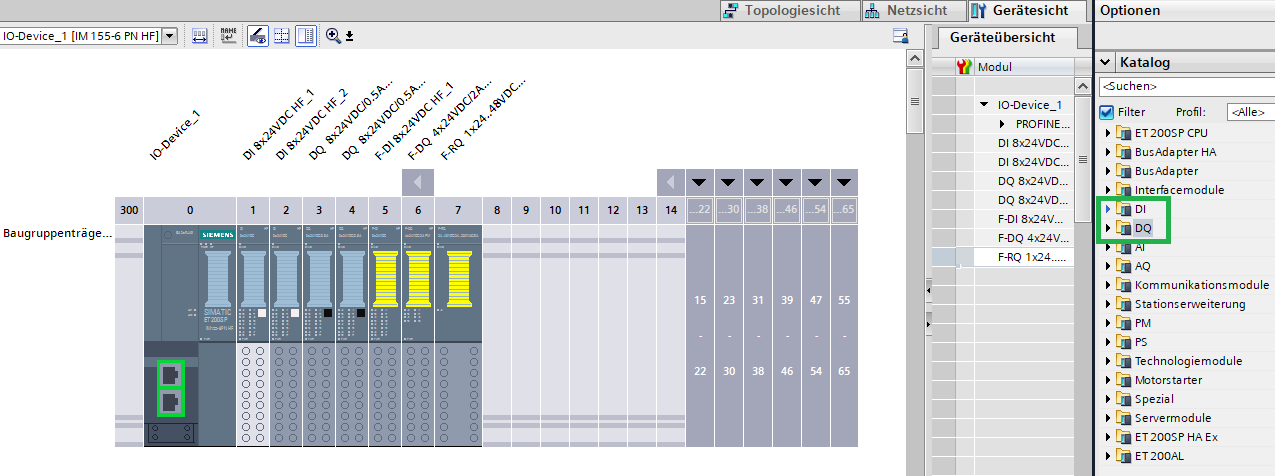
\includegraphics[width=0.9\textwidth]{Bilder/4. Konfiguration der ET 200 SP/4.2 Module hinzufügen/(4.2.2) Elemente der dezentralen Peripherie hinzufuegen.png}}
   \caption[Module hinzufügen]{Module hinzufügen}
   \label{fig:Bild4.4}
\end{figure}

Alle eingefügten Module (bis auf: F-RQ 24VDC/24…230VAC/5A ST) werden zu einer \textbf{Potentialgruppe} hinzugefügt. Dies kann durch das Anklicken der Module und dem anschließenden auswählen von \glqq\textbf{Neue Potentialgruppe ermöglichen (helle BaseUnit)}\grqq\:erfolgen.\\
Pfad: Allgemein > Potentialgruppe

\begin{figure}[H]
   \centering
   \fbox{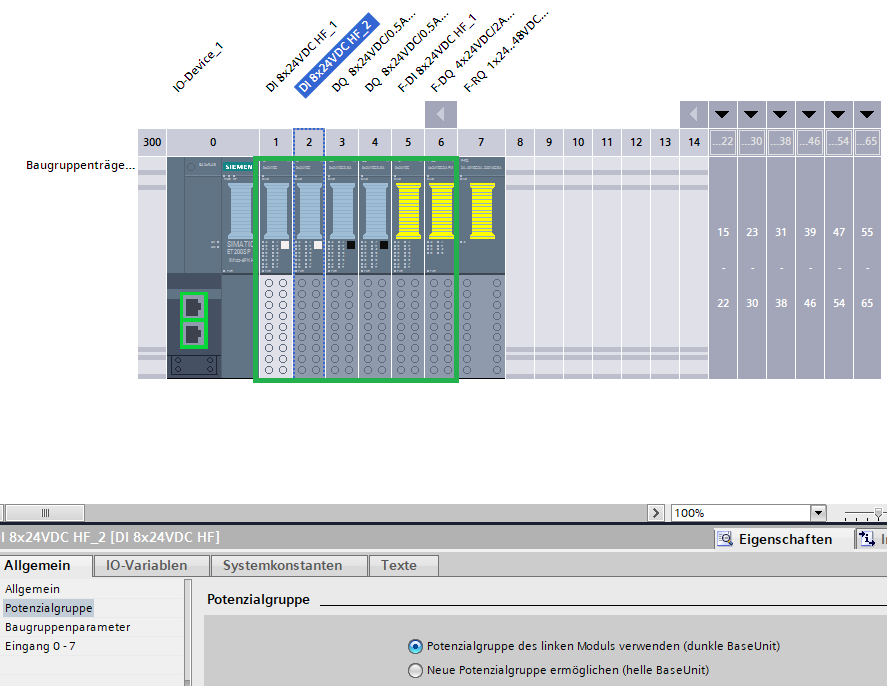
\includegraphics[width=0.75\textwidth]{Bilder/4. Konfiguration der ET 200 SP/4.2 Module hinzufügen/(4.2.3) Potenzialgruppe aendern.png}}
   \caption[Potenzialgruppe anpassen]{Potenzialgruppe anpassen}
   \label{fig:Bild4.5}
\end{figure}

\subsection{Geräteversionen tauschen}
Sofern dies nicht bereits beim Einfügen der Module beachtet wurde, müssen die Versionen des Interfacemoduls IM 155-6PN HF und des Moduls F-DQ angepasst werden. Dies kann durch einen Rechtsklick in der \textbf{Gerätesicht} auf das \glqq\textbf{Modul > Geräte tauschen..}\grqq\:durchgeführt werden. Die Versionsnummern siehe \autoref{tab:Tab4.1}. \\
\textbf{ACHTUNG:} Die Artikel-Nummern müssen übereinstimmen.

\begin{figure}[H]
   \centering
   \fbox{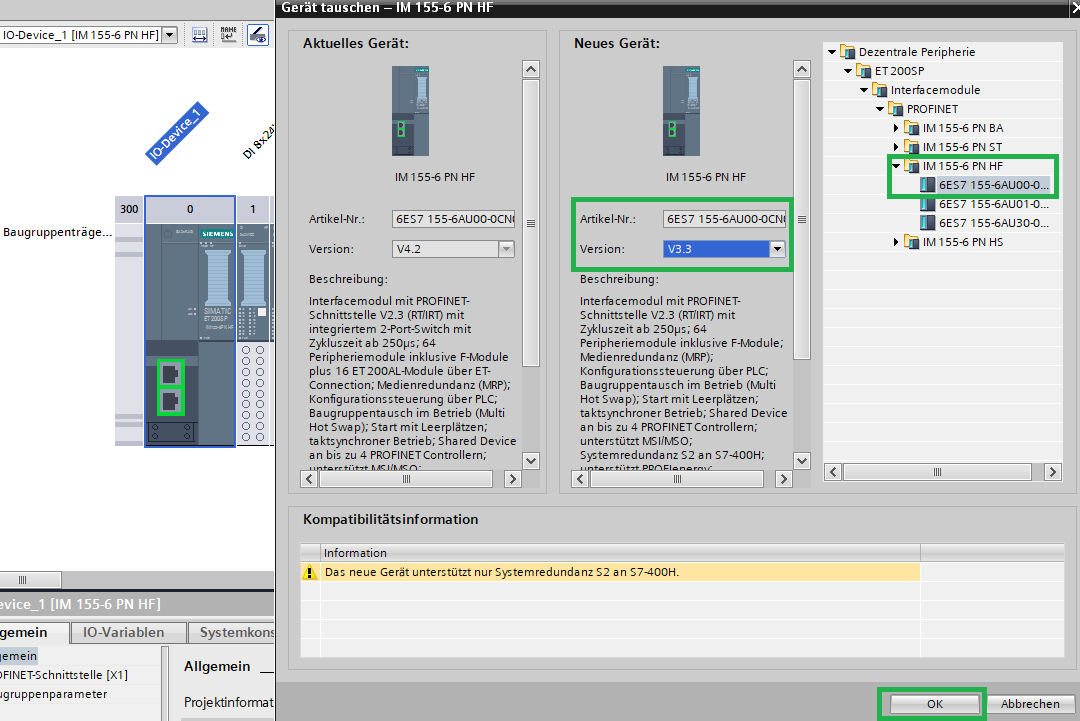
\includegraphics[width=0.65\textwidth]{Bilder/4. Konfiguration der ET 200 SP/4.3 Geräteversionen tauschen/(4.3.1) Geraeteversion tauschen.png}}
   \caption[Geräteversion des IM 155-Interfacemoduls tauschen]{Geräteversion des IM 155-Interfacemoduls tauschen}
   \label{fig:Bild4.6}
\end{figure}

\begin{figure}[H]
   \centering
   \fbox{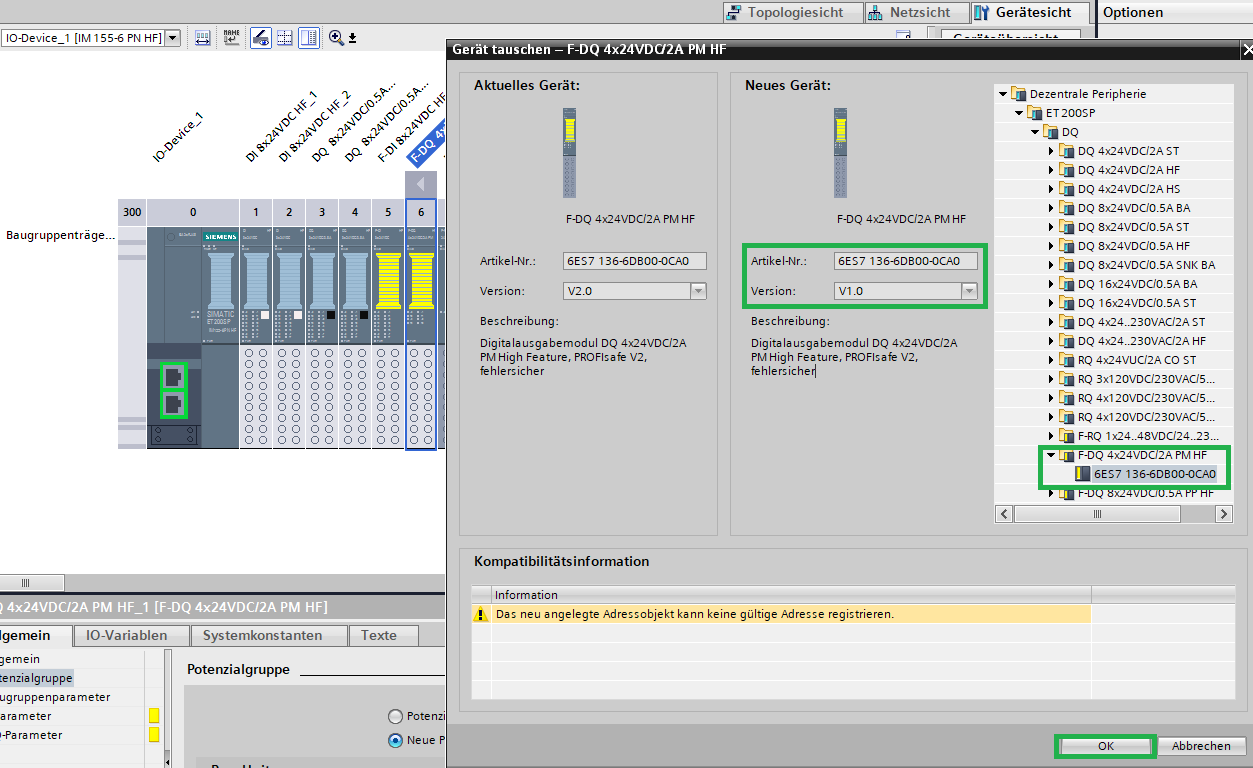
\includegraphics[width=0.65\textwidth]{Bilder/4. Konfiguration der ET 200 SP/4.3 Geräteversionen tauschen/(4.3.2) Geraeteversion tauschen.png}}
   \caption[Geräteversion des F-DQ-Moduls tauschen]{Geräteversion des F-DQ-Moduls tauschen}
   \label{fig:Bild4.7}
\end{figure}

\subsection{IP-Adresse und Vergabe des PROFINET-Gerätenamen der ET 200SP} \label{sec: IP-Adresse_PROFINET-Gerätename_ET_200SP}
Die Bezeichnung der PROFINET-Schnittstelle der ET 200SP ist \textbf{X1}.

\begin{figure}[H]
   \centering
   \fbox{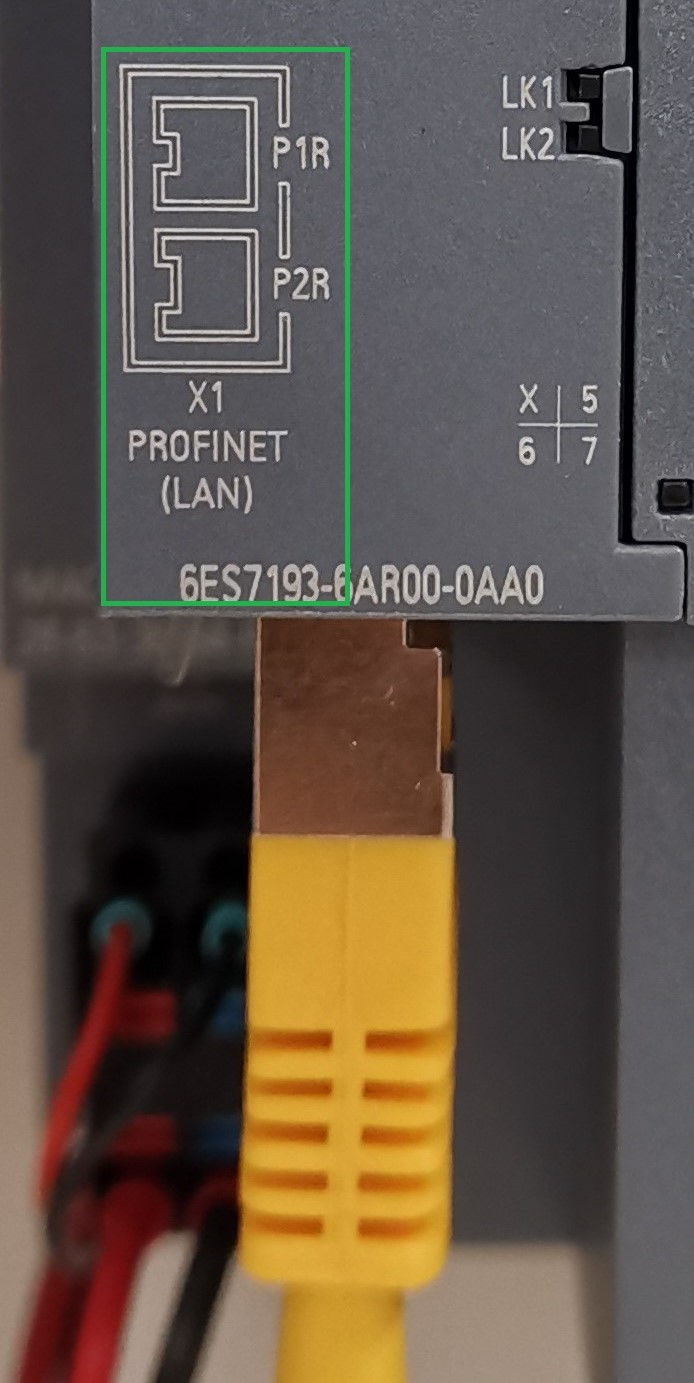
\includegraphics[width=0.2\textwidth]{Bilder/4. Konfiguration der ET 200 SP/4.4 IP-Adresse und Vergabe des PROFINET-Gerätenamen der ET 200 SP/(4.4.1) Bezeichnung der PROFINET-Schnittstelle.jpg}}
   \caption[Bezeichnung der PROFINET-Schnitstelle der ET 200SP]{Bezeichnung der PROFINET-Schnittstelle der ET 200SP}
   \label{fig:Bild4.8}
\end{figure}

Die benötigte IP-Adresse und PROFINET-Gerätename können der \autoref{fig:Bild1.3} entnommen werden. Die Einstellungen sind über die \textbf{Gerätesicht} des Gerätes ET 200SP sichtbar. Bei der Vergabe des PROFINET-Gerätenamens das Häkchen bei \glqq\textbf{PROFINET-Gerätename automatisch generieren}\grqq\:entfernen.\\
Pfad: Allgemein > PROFINET-Schnittstelle [X1]

\begin{figure}[H]
   \centering
   \fbox{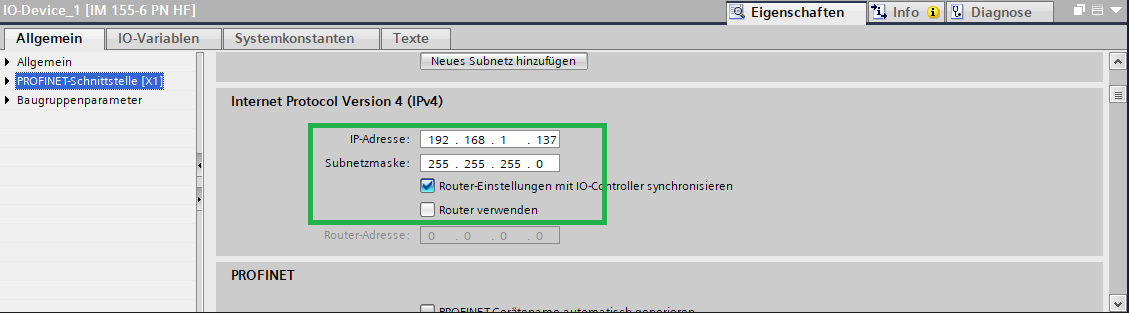
\includegraphics[width=1\textwidth]{Bilder/4. Konfiguration der ET 200 SP/4.4 IP-Adresse und Vergabe des PROFINET-Gerätenamen der ET 200 SP/(4.4.2) IP-Adresse der ET 200 SP.png}}
   \caption[Vergabe der IP-Adresse der ET 200SP]{Vergabe der IP-Adresse der ET 200SP}
   \label{fig:Bild4.9}
\end{figure}

\begin{figure}[H]
   \centering
   \fbox{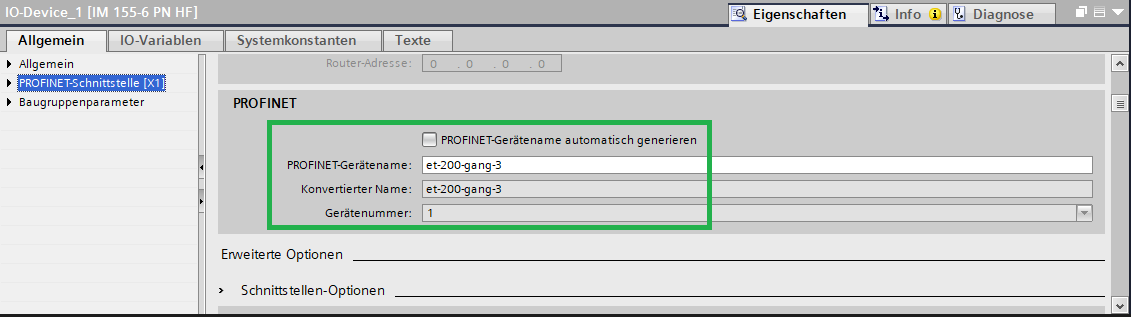
\includegraphics[width=1\textwidth]{Bilder/4. Konfiguration der ET 200 SP/4.4 IP-Adresse und Vergabe des PROFINET-Gerätenamen der ET 200 SP/(4.4.3) PROFINET-Geraetename der ET 200 SP.png}}
   \caption[Vergabe des PROFINET-Gerätenamen der ET 200SP]{Vergabe des PROFINET-Gerätenamen der ET 200SP}
   \label{fig:Bild4.10}
\end{figure}
